\subsubsection{Current language models}
\label{sub:current_language models}

OpenAI made headlines when it first announced the creation of a language model so powerful that it led them to not release it due to ``concerns about malicious applications of the technology''~\footnote{\url{https://openai.com/blog/better-language-models/}}. \gls{gpt2} is a large transformer-based language model with about 1.5 billion parameters, trained on a dataset of 8 million web pages, or 40GB of raw text data~\footcite{radford2019language}. Creators of the \gls{gpt2} model intentionally trained their model on a diverse basis of text in order to produce a \gls{lm} that could generalize well to many different tasks (``zero-shot'' setting) across diverse domains (table~\ref{tab:gpt2_benchmark_scores}) - even outperforming \gls{lm}s trained on specific domains like news or books without needing to use those domain-specific training datasets. What mainly caused the enthusiasm for this model was the fact that it could generate text samples of high, human-like quality and at the same time maintain coherence across long passages of text. After some time passed, OpenAI decided to publish their code, the weights and the training dataset in the form of a staged release. On November 2019, OpenAI released the largest form of their model, also called `GPT-2-XL', consisting of 1.5 billion weights following their releases of the 117M, 345M and 762M parameter-sized models, making it publicly accessible and usable by everyone~\footnote{\url{https://github.com/openai/gpt-2-output-dataset}}.

\begin{table}
	\centering
	\caption{Excerpt of the GPT-2 zero-shot results on different datasets and with different model sizes}
	\begin{tabular}{ cccccccccc }
		\hline
		& LAMBSDA & CBT-CN & WikiText2 & PTB & enwik8 & text8 & WikiText103 & 1BW \\
		& (PPL) & (ACC) & (PPL) & (PPL) & (BPB) & (BPC) & (PPL) & (PPL) \\ \hline
		SOTA & 99.8 & 85.7 & 39.14 & 46.54 & 0.99 & 1.08 & 18.3 & 21.8 \\ \hline
		117M & 35.13 & 87.65 & 29.41 & 65.85 & 1.16 & 1.17 & 37.50 & 75.20 \\
		345M & 15.60 & 92.35 & 22.76 & 47.33 & 1.01 & 1.06 & 26.37 & 55.72 \\
		762M & 10.87 & 93.45 & 19.93 & 40.31 & 0.97 & 1.02 & 22.05 & 44.575 \\
		1542M & 8.63 & 93.30 & 18.34 & 35.76 & 0.93 & 0.98 & 17.48 & 42.16 \\ \hline
	\end{tabular}
	\label{tab:gpt2_benchmark_scores}
\end{table}

Currently there are several language models that are actively being worked on and at the disposal of researchers and interested parties. Especially pretrained models such as \gls{bert}, \gls{gpt2} and XLNet have been known to perform particularly well across common \gls{nlp} tasks. \gls{bert} for instance achieved SotA-scores for Question Answering (SQuAD v1.1), Natural Language Inference (MNLI), and other tasks~\footcite{DBLP:journals/corr/abs-1810-04805}. It is worth noting that both \gls{gpt}-2 as well as \gls{bert} are built on top of the aforementioned transformer architecture proposed by Vaswani and colleagues (subsection~\ref{sub:attention_and_transformers}). \gls{bert} hereby uses the transformer-encoder stack and \gls{gpt2} uses the transformer-decoder stack. The XLNet model presented in mid-2019~\footcite{DBLP:journals/corr/abs-1906-08237} is based on the decoder blocks of a further development of the transformer: Transformer-XL, which extends the transformer architecture by a recurrent connection and a different positional coding~\footcite{DBLP:journals/corr/abs-1901-02860}. \gls{bert} can learn bidirectionally, \gls{gpt}-2 and XLNet unidirectionally using the autoregressive approach. XLNet additionally uses permutation to obtain n representations of the sequence. This allows the model to combine the advantages of autoregression and autoencoding.

Wang and Cho conducted a scientific comparison between the LM performance of the predecessor of \gls{gpt}-2 and \gls{bert}~\footcite{wang2019bert}. The work empirically proves a better quality of \gls{gpt} generation. In contrast, XLNet has recently shown SotA results for problems outside the standard LM task. A scientific comparison of \gls{gpt}-2 and XLNet regarding the classical text generation capability has not yet been made. When comparing the AI community and juxtaposing them in the context of this thesis, the text generation of XLNet seems to be somewhat more coherent, but more often shows grammar errors. Overall, the output of \gls{gpt}-2 slightly exceeds that of XLNet. However, empirical comparisons are necessary to confirm this hypothesis. Another transformer model was recently posted on the GoogleAI blog~\footnote{\url{https://ai.googleblog.com/2020/01/reformer-efficient-transformer.html}}. This transformer is said to have a context window that extends to thousands of words and can thus be used to generate entire Wikipedia articles through multi-document summarization. Google AI researchers believe that the Reformer gives the basis for future use of Transformer models, both for long text and applications outside of natural language processing~\footcite{kitaev2020reformer}. However, as this model was published at the time of an advanced stage of this thesis and as there was no PyTorch implementation of the pretrained model at the time in question, it was not further considered for this thesis. Consequently, the \gls{gpt2} model will be used to generate the text snippets necessary for the later proposed dataset. It is worth mentioning that these \gls{lm}s are freely available to the public. More powerful models created by big tech companies such as the Nvidia \textit{Megatron} with 8.3 billion or the Microsoft \textit{NLG-Turing} with 17 billion parameters do exist (figure~\ref{fig:lm_model_comparison}) but as they are disclosed to the public, no statements can be made about their performance and suitability for this work.
\begin{figure}[h]
  	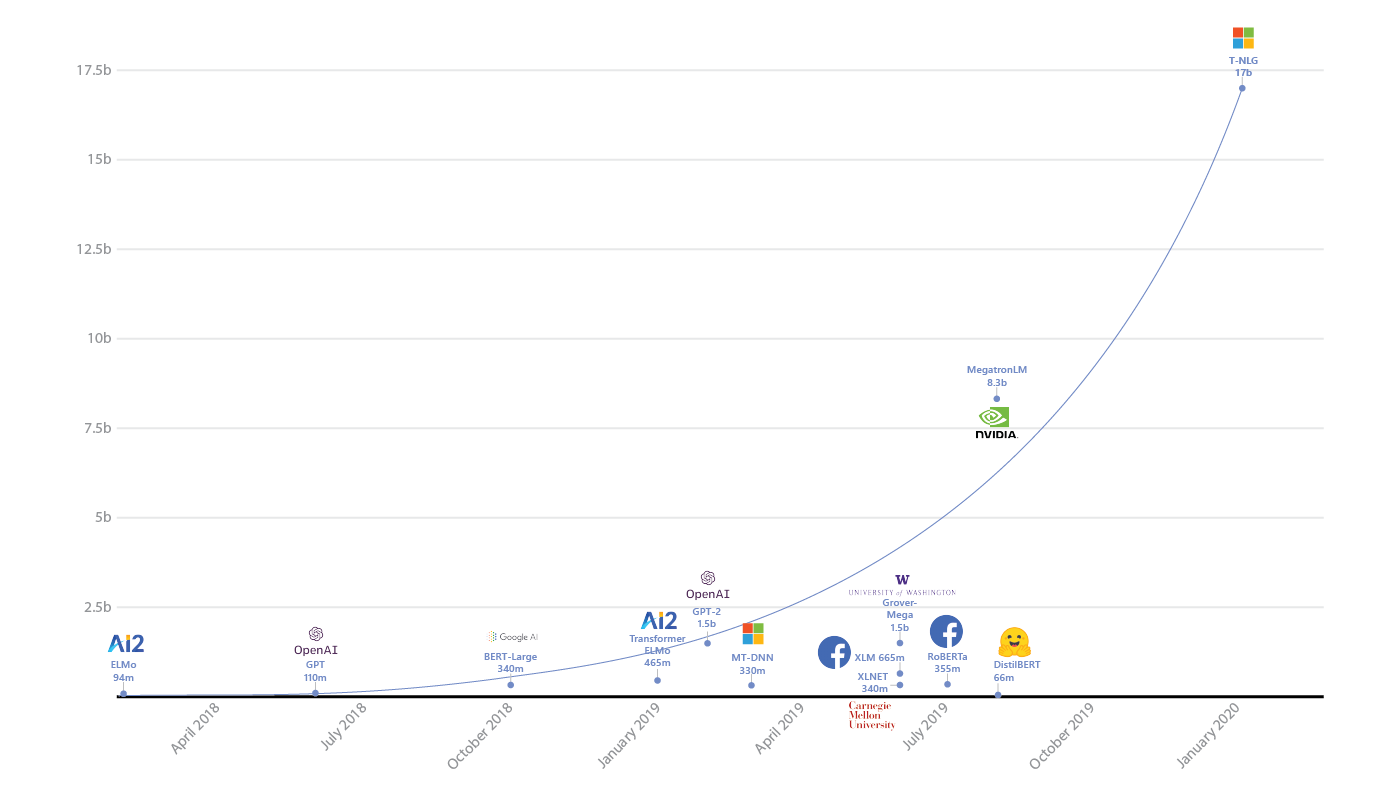
\includegraphics[height=8cm]{img/lm_model_comparison}
  	\caption[Comparison of language model sizes]{Comparison of language model sizes~\footnote{\url{https://www.microsoft.com/en-us/research/blog/turing-nlg-a-17-billion-parameter-language-model-by-microsoft/}}}
	\label{fig:lm_model_comparison}
\end{figure}
